\documentclass[12pt]{article}
\usepackage{geometry}                % See geometry.pdf to learn the layout options. There are lots.
\geometry{letterpaper}                   % ... or a4paper or a5paper or ... 
%\geometry{landscape}                % Activate for for rotated page geometry
\usepackage[parfill]{parskip}    % Activate to begin paragraphs with an empty line rather than an indent
\usepackage{graphicx}
\usepackage{amssymb}
\usepackage{amsthm}
\usepackage{subfig}

\newtheorem{model}{Data-Generating Model}


\title{MCMC inference for qPCR quantitation via branching processes}
\author{Wesley Brooks}
\date{}                                           % Activate to display a given date or no date

\begin{document}
\maketitle

    
\section{Overview}
Bret: because you are quite familiar with may project and its background, I will dispense with some formality in the presentation and get right to the results and discussion.\\

In this project, I use the method presented in \cite{norway:2010} to do inference for a qPCR experiment. The dataset I'll analyze is the Luteinixing Hormone (LH) data that was originally presented in \cite{hanlon:2012}. The experiment was designed as for benchmarking - a cDNA sample was diluted by a factor of 3 and botht the original sample and the diluted sample were run through a qPCR machine. Ideally, our data analysis should recover the known dilution factor. When introducing their analytic method, \cite{norway:2010} used two experiments to justify their results: one was a simulation study and the other an experimental study. But because the experimental study was not controlled in the way I've described above, it was not possible to compare their presented results to a known 'true' dilution.\\


\section{The model}
The data analysis is done via Markov Chain Monte Carlo (MCMC) under the model presented in \cite{norway:2010}. That model is:\\

\textbf{Starting point for the branding process:} $X_{0,j}$ are underlying noiseless starting fluorescences drawn from the starting distribution with mean $\mu_{k_j}$ and precision $\frac{\kappa}{\mu_{k_j}}$ ($j$ indexes the reactions and $k_j$ tells us whether reaction $j$ is under the treatment or control condition):
\[
    X_{0,j}|\mu_{k_j} , \kappa \sim N(\mu_{k_j}, \frac{\kappa}{\mu_{k_j}})
\]


\textbf{Reaction efficiency:} $p_{ij}$ is the probability that each particle will replicate in the $i^{th}$ cycle of reaction $j$. It is fit with a logistic regression model that (I think) fits the decrease in efficiency as the raw materials of the reaction are consumed:
\[
    p_{ij}|X_0 , \alpha_{k_j}, \beta_{k_j}, \tau_p \sim N(\alpha_{k_j} + \beta_{k_j} X_{0,j}\Pi_{i=1}^{m_j-1} (1+p_{ij}), \tau_p)
\]



\textbf{Data:} $Y_{ij}$ are observed fluorescence intensities which are modeled as an underlying fluorescence $X_{ij}$ plus additive noise (precision $=\tau_y$, $i$ indexes the qPCR cycles):
\[
    Y_{ij} \sim N(X_{0,j} \Pi_{i=1}^{m_j} (1+p_{ij}), \tau_y)
\]


\textbf{Prior distributions:} A diffuse Gamma prior is applied to all of the precision parameters ($\tau_p, \tau_y, \kappa$). Gaussian priors are applied to the parameters in the logistic regression models. The priors on the $\mu$ are truncated-Gaussian to ensure the mean is positive. The values of the hyperparameters used in these distributions were exactly the same as those found in \cite{norway:2010}.\\


\section{Data window}
Because the fluorescence $X_0$ is far below the noise threshold, the first several observations are always pure noise. Later the reaction is resource-limited because most of the raw materials have been consumed. Our model is only valid during the exponential-growth phase, between these starting and ending conditions. In the case of the LH data, by eyeball I decided to use cycles 17-20 as the exponential phase for each reaction.\\

The method we're going to use for analysis focuses on the relative fluorescence intensity during the cycle before the exponential phase (e.g., $Y_{1j}$ is the first observation in the exponential phase for reaction $j$, and our inference centers on $X_{0,j}$). If we did not require that the exponential phase began in the same cycle for each reaction (i.e., cycle number 17), then we'd have the messy job of comparing intensities that have not ben amplified the same number of times. So since all of the reactions were in the exponential phase during cycles 17-20, it is simpler to limit our attention to those cycles.\\

\section{Running the algorithm}
Using the model described above and in \cite{norway:2010}, I generated 100,000 draws from the Markov chain, which took about an hour. The first 1000 draws were discarded as the burn-in period, and the remainder were thinned to every $1000^{th}$ draw, leaving 99 ``independent" samples from the posterior distribution. The number of draws was kept relatively small because of time considerations. Convergence of the chain was judged by looking at the trace plots, which looked OK.\\

\section{Results}
The 99 draws from the posterior distribution of the quantitation ratio are plotted in the histogram (Figure \ref{qr}). The median draw is 3.53 and the 95\% credible interval is (2.44, 4.85).

\begin{figure}[hb]
  \centering
  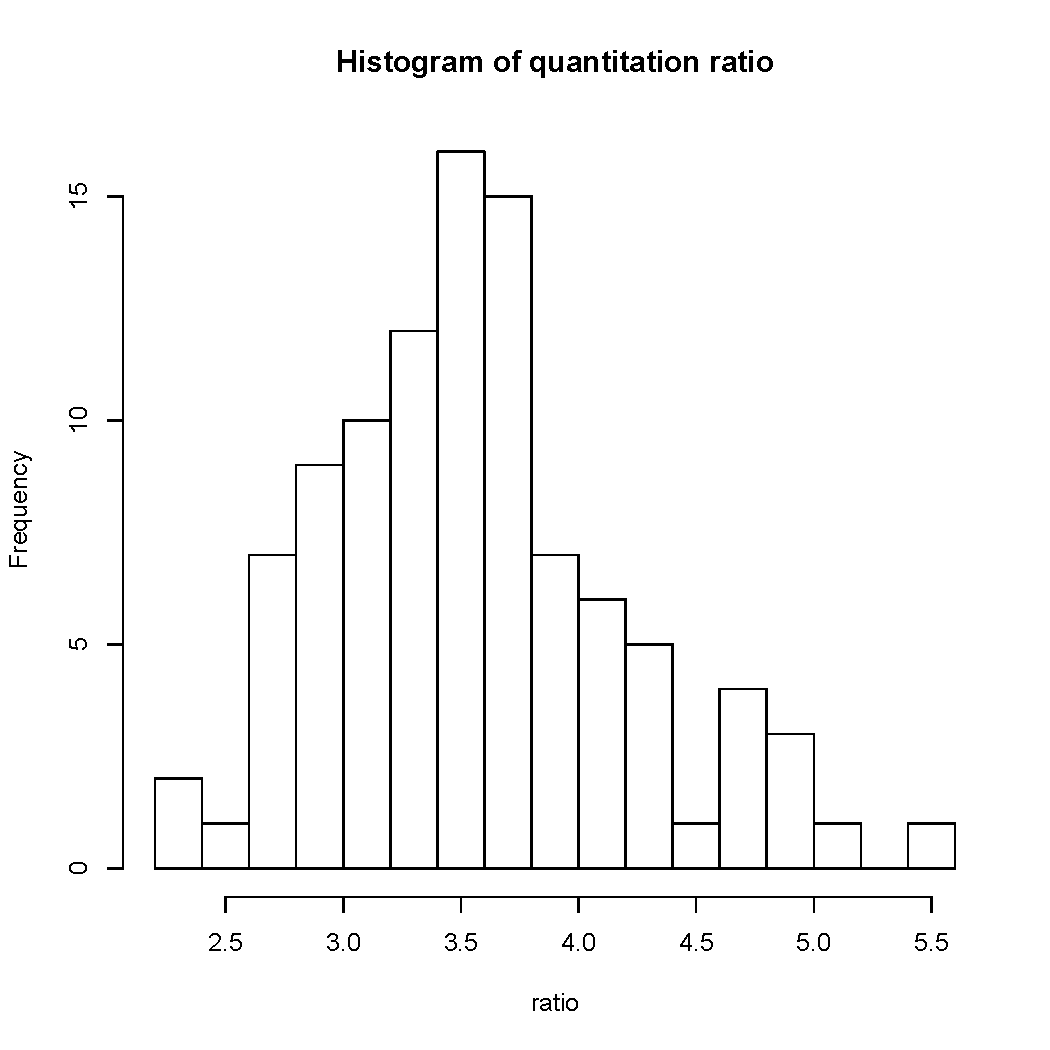
\includegraphics[width=4in]{figures/quantitation_ratio}
  \caption{histogram}
  \label{qr}
\end{figure}

\section{Discussion}
Because our 95\% CI includes the true value of 3, the method appears to be useful for real-life data.

The method used here is described in \cite{norway:2010} as fitting a branching process model. The Norwegian paper \cite{norway:2010} presents two models, though: a ``full" model and a ``simplified" model. The ``full" model is explicitly based on a branching process, but is impractical because the Markov chain failed to converge for the authors in a reasonable time. The ``simplified" model seems to drop the branching process framework: replication is not governed by a binomial random process - instead, the intensity is assumed to grow during each cycle by a factor of $(1+p_{ij})$, with the binomial variability swept into the variability of $p_{ij}$ and $Y_{ij}$. I suspect that one reason the ``full" model failed to converge is that the model for $p_{ij}$ is too flexible, with an error term that is confounded with that of $Y_{ij}$. Using a per-reaction random effect for $p$ may allow convergence of a branching-process-based MCMC algorithm.\\

Inference in this model is not based on the ancestral population of DNA particles - it is based on the population that first emerges above the noise threshold. I think there is a way to use the branching process methodology to augment the observed data with imputed observations from the cycles that are censored by the noise threshold. For instance, in an MCMC setting, we'll have available the latest drawn $p_j$ and know $Y_{ij}$ at the point where it emerges from the noise. Assuming a binomial model for $Y_{ij} | Y_{(i-1)j}$, we can find the likelihood of the possible values of $Y_{(i-1)j}$ and work backward in that way to $Y_{0j}$. Doing so would allow us to drop the ad-hoc windowing, except that we'd still need to ignore the cycles after the reaction is complete.\\


\bibliographystyle{plain}
\bibliography{../references/qpcr}

\end{document}

